\documentclass[leqno]{article}
% Shared QBT/Soln pack preamble for resources.danieljsmith.org.
\usepackage{graphicx}
\usepackage{dsfont}
\usepackage{mathtools}
\usepackage{amssymb}
\usepackage{amsmath}
\usepackage{amsthm}
\usepackage{float}
\usepackage{ragged2e}
\usepackage{tensor}
\usepackage{fancyhdr}
\usepackage{empheq}
\usepackage[most]{tcolorbox}
\usepackage{enumitem}
\usepackage{dirtytalk}
\usepackage{marginnote}
\usepackage{microtype}
\usepackage[
  a4paper,
  left=0.8in,
  right=1in,
  top=1in,
  bottom=0.5in,
  headheight=14pt,
  headsep=0.4in
]{geometry}
\setlength{\parindent}{0cm}

% TikZ / PGFPlots
\usepackage{pgfplots}
\pgfplotsset{compat=1.18}
\usepgfplotslibrary{fillbetween, polar}
\usetikzlibrary{calc, positioning}
\usetikzlibrary{angles, quotes}
\usetikzlibrary{arrows.meta}
\usetikzlibrary{decorations.pathreplacing, decorations.markings}
\usetikzlibrary{patterns}
\usetikzlibrary{intersections}

% Links and contents
\usepackage[colorlinks=true,linkcolor=black,citecolor=magenta,urlcolor=black]{hyperref}%
\urlstyle{same}

% Pack macros
\RenewDocumentCommand{\marks}{o m}{%
  \IfValueTF{#1}%
    {\marginnote{\raggedright\textbf{[#2]}}[#1]}%
    {\marginnote{\raggedright\textbf{[#2]}}}%
}

\newcommand{\vspacerule}[2]{%
  \par\vspace*{#1}%
  \noindent\hrulefill\par
  \vspace*{#2}%
}

\definecolor{scarlet}{RGB}{205, 40, 75}

% Worked-solution box, adapted from the TMUA worked-solutions box. A white breakable box with a left scarlet rule and no surrounding
% frame or tint. A part that breaks fills the rest of its page, so the rule
% runs to the bottom margin; the unbroken or last part ends in a short
% horizontal foot rule so a solution visibly stops. Unlike the TMUA box there
% is no answer label and no extra \parskip: these solutions mix \\ line breaks
% with blank lines, so paragraph skips would make the spacing uneven. The box
% does not grow to the left, so the rule sits at the text edge; growing to the
% right keeps the usable line width close to the old tcolorbox Solution box.
\newtcolorbox{djsSolution}{%
  enhanced, breakable, frame hidden, sharp corners, colback=white,
  height fixed for=first and middle, height fill,
  extras unbroken and last={natural height},
  borderline west={2.2pt}{0pt}{scarlet},
  left=11pt, right=0pt, top=5pt, bottom=13pt,
  before skip=13pt, after skip=4pt,
  grow to right by=10mm,
  overlay unbroken and last={%
    \fill[scarlet] (frame.south west)
      rectangle ([xshift=3.5cm, yshift=2.2pt]frame.south west);},
  before upper={{\color{scarlet}\bfseries Solution}\par\vspace{4pt}}}

% Optional smaller figure inside a solution box. \scalebox shrinks node text
% with the drawing. Not applied to existing figures.
\newcommand{\SolnFigureScale}{0.85}
\newsavebox{\djsSolnFigureBox}
\newenvironment{djsSolutionFigure}
  {\par\vspace{4pt}\begin{center}\begin{lrbox}{\djsSolnFigureBox}}
  {\end{lrbox}\scalebox{\SolnFigureScale}{\usebox{\djsSolnFigureBox}}%
   \end{center}\vspace{2pt}\par}

\newcommand{\cxl}[2]{%
  \tikz[baseline=(X.base)]{%
    \node[inner sep=0pt, outer sep=0pt, text=#1] (X) {$#2$};
    \draw[#1, line width=0.4pt] (X.south west)--(X.north east);
  }%
}

% Page-style hook run at the contents page and each question's opening page.
% A no-op for QBT packs; \djsSolnHeader points it at the fancy header.
\newcommand{\djsQuestionPageStyle}{}

\newcommand{\questionitem}{%
  \djsQuestionPageStyle
  \item\phantomsection
  \addcontentsline{toc}{section}{Question \number\value{enumi}}%
}

\renewcommand{\contentsname}{Questions}

\newcommand{\djsPackHeader}[1]{%
  \pagestyle{fancy}%
  \fancyhead{}%
  \fancyfoot{}%
  \renewcommand{\headrulewidth}{0.9pt}%
  \lhead{#1}%
  \chead{}%
  \rhead{\href{https://danieljsmith.org}{danieljsmith.org}}%
}

\newcommand{\djsQbtHeader}[1]{%
  \djsPackHeader{#1}%
}

% Solutions packs show the header only on the contents page and each
% question's opening page, so it never appears part-way through a solution.
% \thispagestyle marks the next page shipped out, which is the question's
% page because every solution question starts after a \newpage.
\newcommand{\djsSolnHeader}[1]{%
  \djsPackHeader{\textit{Solutions} - #1}%
  \pagestyle{empty}%
  \renewcommand{\djsQuestionPageStyle}{\thispagestyle{fancy}}%
}

\newcommand{\djsFrontMatter}{%
  \djsQuestionPageStyle
  \vspace*{20pt}%
  \tableofcontents
  \newpage
}


\djsQbtHeader{Power and Driving Force}

\begin{document}
\djsFrontMatter
\begin{enumerate}[
  label=\textbf{\arabic*.},
  leftmargin=*,
  topsep=0pt,
  partopsep=0pt,
  parsep=0pt
]


% ---- Question 1 ----
\questionitem
% [Source: _QBT___Power_and_Driving_Force_, Q1]

A delivery van of mass $2000\,\mathrm{kg}$ is travelling up a straight road inclined at angle $\alpha$ to the horizontal, where $\sin\alpha=0.05$. \\

The van's engine can produce power at a maximum rate of $64\,\mathrm{kW}$. \\

The total resistance force due to friction and air resistance is modelled as $(200+kv)\,\mathrm{N}$, where $v\,\mathrm{m\,s^{-1}}$ is the speed of the van and $k$ is a constant. \\

The greatest possible constant speed of the van up the hill is $20\,\mathrm{m\,s^{-1}}$. \\

Find the maximum possible acceleration of the van when it is travelling uphill at $16\,\mathrm{m\,s^{-1}}$. \\

Fully justify your answer. \marks{7} \\

\newpage

% ---- Question 2 ----
\questionitem
% [Source: _QBT___Power_and_Driving_Force_, Q2]

A delivery van has mass $1300\,\mathrm{kg}$ and travels on a straight horizontal road. \\

In a simple model, the van experiences a constant rolling resistance of $600$ newtons and an additional air-resistance force whose magnitude is proportional to the speed of the van. \\

During a test, the van moves at a steady speed of $15\,\mathrm{m\,s^{-1}}$ when the engine provides a driving force of $1200$ newtons. \\

In this model, the engine can deliver a constant maximum power. The greatest speed the van can attain on this road is $30\,\mathrm{m\,s^{-1}}$. \\

\begin{enumerate}[label=\textbf{(\alph*)}]
  \item Show that the maximum power of the engine is $54\,000\,\mathrm{W}$ \marks{2} \\
  \item Find the maximum acceleration of the van when it is travelling at $20\,\mathrm{m\,s^{-1}}$ \marks{3} \\
  \item Find the maximum acceleration of the van when it is travelling at $4\,\mathrm{m\,s^{-1}}$ \marks{1} \\
  \item Comment on the validity of the model in the context of your answers to parts (b) and (c). \marks{2} \\
\end{enumerate}

\newpage

% ---- Question 3 ----
\questionitem
% [Source: _QBT___Power_and_Driving_Force_, Q3]

A maintenance vehicle of mass $1000\,\mathrm{kg}$ moves on a straight slope inclined at an angle $\theta$ to the horizontal, where $\sin\theta=0.08$. When the motor is switched off, the vehicle coasts down the slope and reaches a limiting speed of $14\,\mathrm{m\,s^{-1}}$. The resistance to motion is proportional to the square of the speed. The motor is then switched on and works at a constant power $P\,\mathrm{W}$, allowing the vehicle to travel up the same slope with a limiting speed of $10\,\mathrm{m\,s^{-1}}$. \\

Find the value of $P$ and determine the resistance to motion when the vehicle is travelling at $12\,\mathrm{m\,s^{-1}}$ \marks{10} \\

\newpage

% ---- Question 4 ----
\questionitem
% [Source: _QBT___Power_and_Driving_Force_, Q4]

\begin{figure}[H]
    \centering
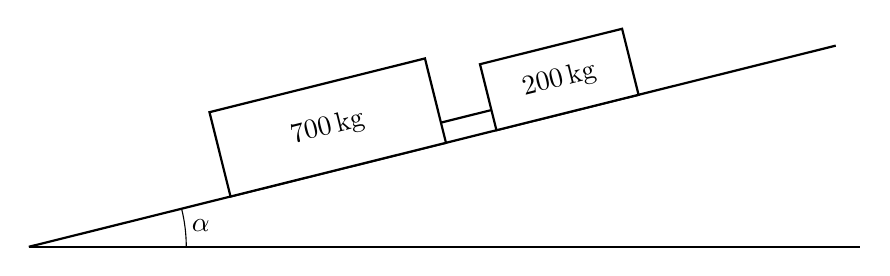
\begin{tikzpicture}[scale=1.2]
\def\ang{14}
\def\planelen{8.8}
\def\carx{2.2}
\def\clen{2.35}
\def\cheight{0.92}
\def\tlen{1.55}
\def\theight{0.72}
\def\gap{0.55}
\def\hitchh{0.22}
\pgfmathsetmacro{\trailx}{\carx+\clen+\gap}

\coordinate (A) at (0,0);
\coordinate (B) at (\ang:\planelen);
\coordinate (H) at (\planelen,0);
\coordinate (Cpos) at (\ang:\carx);
\coordinate (Tpos) at (\ang:\trailx);

\draw[thick] (A) -- (B);
\draw[thick] (A) -- (H);
\pic["$\alpha$", draw, angle radius=20mm, angle eccentricity=1.1] {angle=H--A--B};

\begin{scope}[shift={(Cpos)}, rotate=\ang]
  \coordinate (CarTow) at (\clen,\hitchh);
  \draw[thick, fill=white] (0,0) rectangle (\clen,\cheight);
  \node[rotate=\ang] at ({0.5*\clen},{0.5*\cheight}) {$700\,\mathrm{kg}$};
\end{scope}

\begin{scope}[shift={(Tpos)}, rotate=\ang]
  \coordinate (TraTow) at (0,\hitchh);
  \draw[thick, fill=white] (0,0) rectangle (\tlen,\theight);
  \node[rotate=\ang] at ({0.5*\tlen},{0.5*\theight}) {$200\,\mathrm{kg}$};
\end{scope}

\draw[thick] (CarTow) -- (TraTow);
\end{tikzpicture}
\end{figure}


A car of mass $700\,\mathrm{kg}$ is descending a straight road which is inclined at an angle $\alpha$ to the horizontal, where $\sin\alpha=\tfrac{1}{10}$. The car is connected to a trailer of mass $200\,\mathrm{kg}$ by a light rigid towbar which is parallel to the road, as shown in the diagram. \\

The resistance to the motion of the car is modelled as a constant force of magnitude $240\,\mathrm{N}$. 

The resistance to the motion of the trailer is modelled as a constant force of magnitude $90\,\mathrm{N}$. \\

The brakes of the car dissipate energy at a constant rate of $9\,\mathrm{kW}$. \\

Find the force in the towbar at the instant when the speed of the car is $12\,\mathrm{m\,s^{-1}}$, stating whether the towbar is in tension or compression. \marks{8} \\

\newpage

% ---- Question 5 ----
\questionitem
% [Source: _QBT___Power_and_Driving_Force_, Q5]

An airport tug of mass $1800\,\mathrm{kg}$ has an engine that can deliver a maximum power of $72\,\mathrm{kW}$. \\

In an initial model of the motion of the tug, the total resistance to motion is assumed to be constant. \\

\begin{enumerate}[label=(\roman*)]
  \item Given that the greatest steady speed of the tug on a straight horizontal runway is $18\,\mathrm{m\,s^{-1}}$, find the magnitude of the resistance force. \marks{2} \\
  \item The tug is connected to a small aircraft of mass $2200\,\mathrm{kg}$ by a light rigid horizontal tow bar. The greatest steady speed of the tug and aircraft on the runway is now $12\,\mathrm{m\,s^{-1}}$. The resistance to motion of the aircraft may also be assumed constant. \\

  Find the magnitude of the resistance force on the aircraft. \marks{2} \\
  \item The tug and aircraft again travel along the runway. At one instant their speed is $10\,\mathrm{m\,s^{-1}}$ and their acceleration is $0.25\,\mathrm{m\,s^{-2}}$. \\

  \begin{enumerate}[label=(\alph*)]
    \item Find the power of the engine of the tug at this instant. \marks{4}
    \item Find the magnitude of the force in the tow bar at this instant. \marks{2}\\
  \end{enumerate}
  \item In a refined model of the motion of the tug and aircraft, the resistance to motion of each is assumed to be zero until they reach a speed of $6\,\mathrm{m\,s^{-1}}$. When the speed is $6\,\mathrm{m\,s^{-1}}$ or above, the same constant resistance forces as in the first model are assumed to apply to each. \\

  The tug and aircraft start from rest on the runway and accelerate, using maximum power. \\

  Without carrying out any further calculations,
  \begin{enumerate}[label=(\alph*)]
    \item explain whether the time taken to attain a speed of $10\,\mathrm{m\,s^{-1}}$ would be predicted to be lower, the same or higher using the refined model compared with the original model. \marks{2}
    \item explain whether the greatest steady speed of the system would be predicted to be lower, the same or higher using the refined model compared with the original model. \marks{2}
  \end{enumerate}
\end{enumerate}

\newpage

% ---- Question 6 ----
\questionitem
% [Source: _QBT___Power_and_Driving_Force_, Q6]

A snowmobile of mass $800\,\mathrm{kg}$ tows a rescue sledge of mass $200\,\mathrm{kg}$ up a straight slope that is inclined at angle $\theta$ to the horizontal. The sledge is attached to the snowmobile by a light inextensible rope. The resistance to the motion of the snowmobile from non-gravitational forces is modelled as a constant force of magnitude $216\,\mathrm{N}$. The resistance to the motion of the sledge from non-gravitational forces is modelled as a constant force of magnitude $294\,\mathrm{N}$. \\

When the engine of the snowmobile is working at a constant rate of $12\,\mathrm{kW}$, the snowmobile and the sledge move up the slope with constant speed $12\,\mathrm{m\,s^{-1}}$. \\

\begin{enumerate}[label=\textbf{(\alph*)}]
  \item Find the value of $\sin\theta$. \marks{4} \\
  \item Later, at the instant when the snowmobile and the sledge are travelling down the slope with speed $14\,\mathrm{m\,s^{-1}}$, the rope snaps. When the rope snaps the sledge is at the point $A$. The sledge continues to travel down the slope before coming to instantaneous rest at the point $B$. The resistance to the motion of the sledge from non-gravitational forces is again modelled as a constant force of magnitude $294\,\mathrm{N}$. \\

  Use the work-energy principle, and your answer to part (a), to find the distance $AB$. \marks{5} \\
\end{enumerate}

\newpage

% ---- Question 7 ----
\questionitem
% [Source: _QBT___Power_and_Driving_Force_, Q7]

A lorry of mass $3200\,\mathrm{kg}$ tows a trailer of mass $1800\,\mathrm{kg}$ down a line of greatest slope of a straight road inclined at an angle $\theta$ to the horizontal, where $\sin\theta=0.06$. \\

The power developed by the lorry's engine is constant. The resistances to motion of the lorry and the trailer are constant and equal to $800\,\mathrm{N}$ and $500\,\mathrm{N}$ respectively. When the lorry passes through a point $A$ on the road, the speed of the combination is $14\,\mathrm{m\,s^{-1}}$ and its acceleration is $1.2\,\mathrm{m\,s^{-2}}$. \\

\begin{enumerate}[label=\textbf{(\alph*)}]
  \item Calculate the power developed by the engine. \marks{5} \\
  \item The lorry later passes through a point $B$ on the road with speed $22\,\mathrm{m\,s^{-1}}$. The time taken for the lorry to travel from $A$ to $B$ is $7.93\,\mathrm{s}$. \\

  Find the distance $AB$. \marks{5} \\
\end{enumerate}

\newpage

% ---- Question 8 ----
\questionitem
% [Source: _QBT___Power_and_Driving_Force_, Q8]

A lorry of mass $2500\,\mathrm{kg}$ travels up a straight road inclined at an angle $\alpha$ to the horizontal, where $\tan\alpha=\dfrac{7}{24}$. \\

The engine of the lorry supplies a constant power of $P\,\mathrm{W}$. The total resistance to motion is a constant force of magnitude $R\,\mathrm{N}$. \\

When the lorry is moving at $12\,\mathrm{m\,s^{-1}}$, its acceleration is $2.4\,\mathrm{m\,s^{-2}}$. When it is moving at $18\,\mathrm{m\,s^{-1}}$, its acceleration is $0.4\,\mathrm{m\,s^{-2}}$. \\

Find the value of $P$ and the value of $R$ \marks{8} \\

\newpage

% ---- Question 9 ----
\questionitem
% [Source: _QBT___Power_and_Driving_Force_, Q9]

A van of mass $1000\,\mathrm{kg}$ is driven up a straight road inclined at an angle $\alpha$ to the horizontal, where $\sin\alpha=\dfrac{1}{20}$. The engine is working at a constant rate of $12\,\mathrm{kW}$ and the van moves at a constant speed of $15\,\mathrm{m\,s^{-1}}$. \\

\begin{enumerate}[label=\textbf{(\alph*)}]
  \item Find the resistance to the motion of the van. \marks{4} \\
  \item The van now tows a trailer of mass $600\,\mathrm{kg}$ up the same road using a tow rope parallel to the line of motion. The resistance to the motion of the van is the same as in part (a), and the resistance to the motion of the trailer is a constant force of magnitude $106\,\mathrm{N}$. \\

  The engine is still working at a constant rate of $12\,\mathrm{kW}$. \\

  The tow rope is modelled as light and inextensible. \\

  Using the model, find the tension in the tow rope at the instant when the speed of the van is $7.5\,\mathrm{m\,s^{-1}}$. \marks{5} \\
\end{enumerate}

\newpage

% ---- Question 10 ----
\questionitem
% [Source: _QBT___Power_and_Driving_Force_, Q10]

A lorry of mass $2400\,\mathrm{kg}$ is towing a trailer of mass $600\,\mathrm{kg}$ up a straight road inclined at an angle $\theta$ to the horizontal, where $\sin\theta=\dfrac{1}{49}$. \\

When the lorry and trailer move at speed $v\,\mathrm{m\,s^{-1}}$, the total resistance to motion has magnitude $(300+60v)\,\mathrm{N}$. \\

The greatest constant speed that the lorry and trailer can maintain on this hill is $15\,\mathrm{m\,s^{-1}}$. \\

Find the maximum power output of the lorry's engine. \\

Fully justify your answer. \marks{5} \\

\newpage

% ---- Question 11 ----
\questionitem
% [Source: _QBT___Power_and_Driving_Force_, Q11]

A maintenance train has mass $10\,000\,\mathrm{kg}$ and the maximum power of its engine is $200\,\mathrm{kW}$. In a model of the train's motion, it is assumed that while the train is moving the total resistance to motion is constant. \\

On a straight horizontal track, the greatest constant speed that the train can maintain when the engine is working at maximum power is $20\,\mathrm{m\,s^{-1}}$. \\

\begin{enumerate}[label=\textbf{(\alph*)}]
  \item Find the resistance to motion. \marks{2} \\
  \item While the train is still on horizontal track, the engine is delivering $60\,\mathrm{kW}$ when the speed of the train is $8\,\mathrm{m\,s^{-1}}$. \\
  Find the acceleration of the train at this instant. \marks{2} \\
  \item The train then climbs a straight track inclined at an angle $\theta$ above the horizontal. When the engine is working at maximum power, the greatest constant speed that the train can maintain is $10\,\mathrm{m\,s^{-1}}$. \\
  Determine the value of $\theta$. \marks{3} \\
\end{enumerate}

\newpage

% ---- Question 12 ----
\questionitem
% [Source: _QBT___Power_and_Driving_Force_, Q12]

A rail maintenance vehicle of mass $2000\,\mathrm{kg}$ travels in a straight line along a horizontal section of track at a constant speed of $20\,\mathrm{m\,s^{-1}}$. \\

The resistance to the motion of the vehicle is modelled as a constant force of magnitude $2000\,\mathrm{N}$. \\

The engine is working at a constant rate of $P\,\mathrm{kW}$. \\

Using the model, \\

\begin{enumerate}[label=\textbf{(\alph*)}]
  \item find the value of $P$. \marks{3} \\
\end{enumerate}

The vehicle now travels up a straight section of track which is inclined to the horizontal at an angle $\alpha$, where $\sin \alpha = \dfrac{1}{20}$. \\

In a refined model, the resistance to the motion of the vehicle from non-gravitational forces is modelled as a force of magnitude $(220 + 2v^2)\,\mathrm{N}$, where $v\,\mathrm{m\,s^{-1}}$ is the speed. \\

At the instant when the engine is working at the same constant rate as in part (a) and the vehicle is moving up the track at $10\,\mathrm{m\,s^{-1}}$, the acceleration of the vehicle is $a\,\mathrm{m\,s^{-2}}$. \\

Using the refined model, \\

\begin{enumerate}[label=\textbf{(\alph*)}, resume]
  \item find the value of $a$. \marks{4} \\
\end{enumerate}

Later, when the engine is again working at this constant rate, the vehicle is moving up the track at a constant speed $U\,\mathrm{m\,s^{-1}}$. \\

Using the refined model, \\

\begin{enumerate}[label=\textbf{(\alph*)}, resume]
  \item find the value of $U$. \marks{5} \\
\end{enumerate}
\end{enumerate}
\end{document}
